\clearpage  % move to another page
\begin{appendices}
%   The following sections include images of the transpiled circuits on the
%   different backends, followed by the code used to implement the circuits and
%   sample output.
  \clearpage % move to another page

\section*{Transpiled Circuits}
\begin{figure*}
  % \centering
  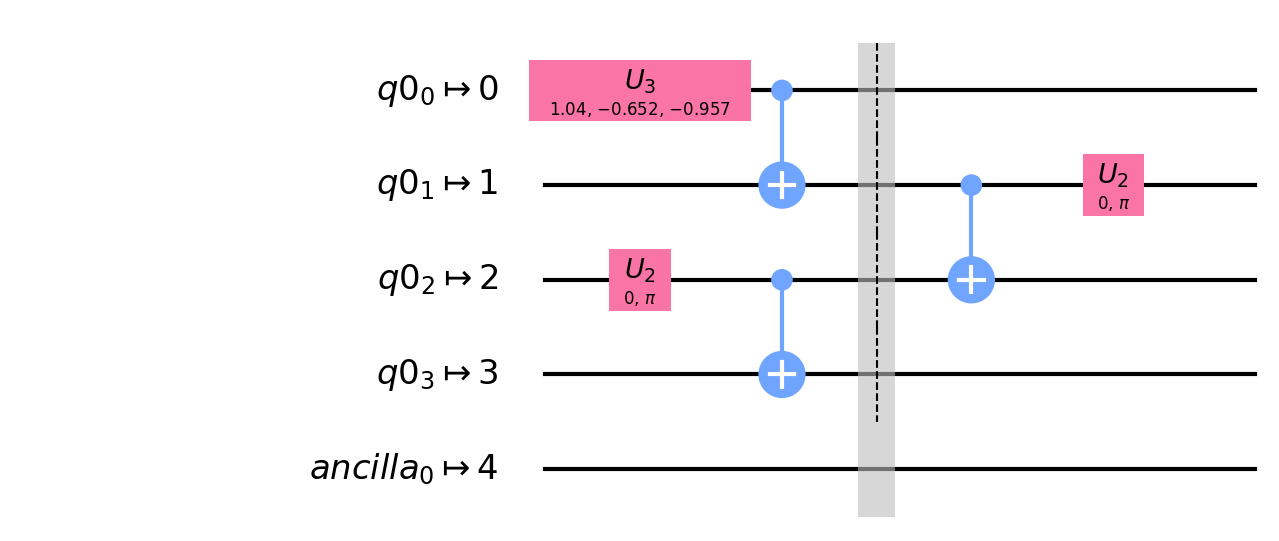
\includegraphics[width=0.6\textwidth]{images/swap_ibmqx2.png}
  \caption{Implementing swap on the Yorktown and Melbourne backends use the
    minimal number of gates.}
  \label{fig:swap_york_trans}
\end{figure*}
  
\begin{figure*}
  \centering
  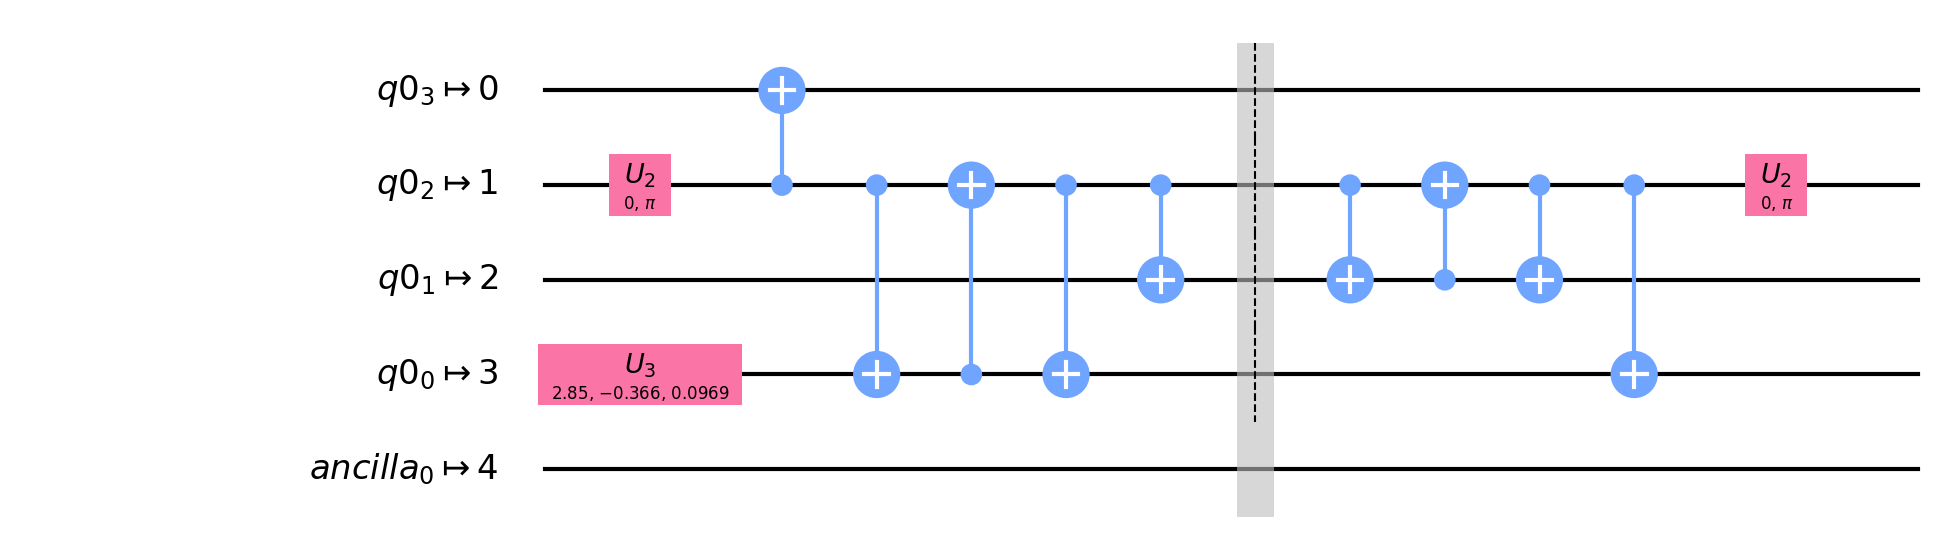
\includegraphics[width=\textwidth]{images/swap_burlington.png}
  \caption{The implementation of the swapping protocol requires many more
    2-qubit gates on the Burlington device due to it T-shape and low
    inter-connectivity. This circuit should be compared to Fig.
    \ref{fig:swap_york_trans}, with just three CNOT gates.}
  \label{fig:swap_burl_trans}
\end{figure*}

\end{appendices}

%%% Local Variables:
%%% mode: latex
%%% TeX-master: "report"
%%% End: